\section{Бесперапынная інтэграцыя і дастаўка}

\subsection{Асноўныя паняцці}

Бесперапынная інтэграцыя азначае, што зборка і тэсціраванне (Unit-testing)
праграмнага забеспячэння адбываюцца аўтаматычна і часта.
Частата азначае, зборка праграмнага забеспячэння адбываецца перыядычна
альбо, напрыклад, пры кожным змяненні ў кантролі версій змяненняў.
Заўважым, што ключавым момантам ў бесперапыннай інтэграцыі з'яўляецца тое,
што працэс тэсціравання (інтэграцыя праграмнага забеспячэння) аўтаматызаваны
пры дапамозе інструментаў і не патрабуе ручнога ўмяшання падчас
зборкі і тэсціравання%
[\ref{book:Continuous Integration}].

Бесперапынная дастаўка азначае, што праграмнае забеспячэнне
заўсёды гатовае да разгортвання.
Праграмнае забеспячэнне збіраецца і тэсціруецца падчас працэсаў
бесперапыннай інтэграцыі і, таксама, разгортваецца ў адмысловае
асяроддзе для далейшых тэстаў.
Ключавым момантаў у бесперапыннай дастаўцы з'яўляецца тое,
што кожная версія зборкі аўтаматычна правяраецца на гатоўнасць да
разгортвання[\ref{book:Continuous Delivery}].

Бесперапыннае разгортванне азначае аўтаматычнае разгортванне
праграмнага забеспячэння ў вытворчасць пасля таго, як
унесены змены ў вытворчую галіну кантроля версіі і паспяхова пройдзены
аўтаматычныя тэсты на праверку гатоўнасці да разгортвання.
Зборка, тэсціраванне, разгортванне ажыццяўляюцца без ўмяшання чалавека%
[\ref{book:Continuous Delivery vs. Continuous Deployment}].

Такім чынам адрозненнем паміж бесперапыннай дастаўкай і разгортваннем
з'яўляецца тое, што пры працэсе бесперапыннай дастаўкі праграмнае
забеспячэнне сцвярджаецца гатовым да разгортвання ў вытворчасць чалавекам.
У той жа час пры працэсе бесперапыннага разгортвання праграмнае
забеспячэнне аўтаматычна разгортваецца ў вытворчасць.

Бесперапынная дастаўка і разгортванне часта памылкова ўжываюцца як
сінонімы, аднак неабходна разумець, што розніца паміж гэтымі двума
тэрмінамі існуе. На малюнку \ref{figure:relations of CI, CD, CD}
прадстаўлены ўзаемаадносіны паміж бесперапыннай інтэграцыяй, дастаўкаў і
разгортваннем.

\begin{figure}[h!]
    \centering
    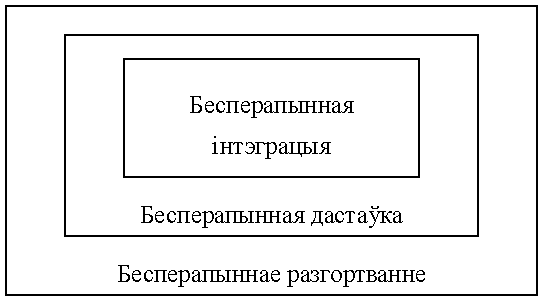
\includegraphics{Relations_of_CI_CD_CD.pdf}
    \caption{Узаемаадносіны паміж бесперапыннай
             інтэграцыяй, дастаўкай і разгортваннем}
    \label{figure:relations of CI, CD, CD}
\end{figure}

Згодна з малюнкам \ref{figure:relations of CI, CD, CD}
можна сцвярджаць, што немагчыма пабудаваць канвеер бесперапыннага
разгортвання без працэсаў бесперапыннай інтэграцыі і дастаўкі,
так як адно ўключае другое.

На малюнку \ref{figure:Difference_between_CD_and_CD}
прадстаўлены канвееры бесперапыннай дастаўкі і разгортвання.

\begin{figure}[h!]
    \centering
    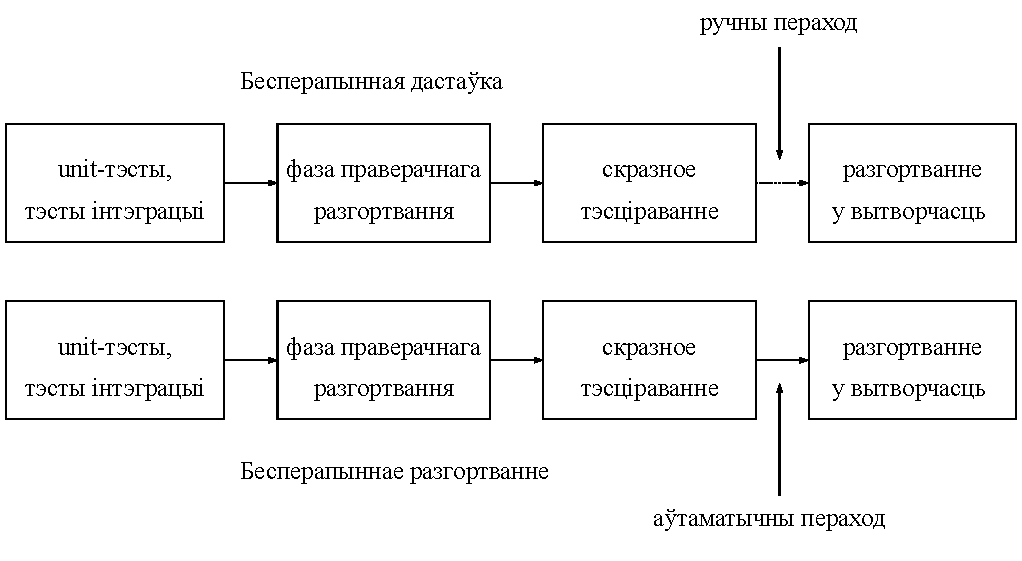
\includegraphics[width=\linewidth]{Difference_between_CD_and_CD.pdf}
    \caption{Адрозненне паміж бесперапыннай дастаўкай і разгортваннем}
    \label{figure:Difference_between_CD_and_CD}
\end{figure}

Падвядзем ітог тэрміналогіі:
\begin{enumerate}
    \item Бесперапынная інтэграцыя -- гэта набор практык,
          мэта каторага паляпшэнне якасці і хуткасці распрацоўкі
          праграмнага забеспячэння пры дапамозе аўтаматызацыі
          зборкі і тэсціравання, а таксама памяншэнне імавернасці
          памылак праз ручную зборку альбо праз розныя
          ўласцівасці асяроддзя выканання зборкі.
          Бесперапынная інтэграцыя з'яўляецца часткай бесперапыннай
          дастаўкі;
    \item Бесперапынная дастаўка -- гэта набор практык,
          які ўключае ў сябе бесперапынную інтэграцыю і дадае 
          да яе аўтаматызацыю скразнога тэсціравання і дастаўку
          праграмнага забеспячэння такім чынам, каб канчатковая
          зборка праграмы магла прымяняцца на патрэбных платформах
          і пры пэўных умовах.
          Бесперапынная дастаўка з'яўляецца часткай бесперапыннага
          разгортвання і не ўключае ў сябе аўтаматычнае
          разгортванне праграмнага забеспячэння ў вытворчасць;
    \item Бесперапыннае разгортванне -- гэта набор практык, які
          ўключае ў сябе вышэй узгаданыя бесперапынную інтэграцыю
          і дастаўку, аднак дадае да іх аўтаматычнае разгортванне
          праграмнага забеспячэння ў вытворчасць.
          Пры ідэальных умовах, канвеер бесперапыннага разгортванне
          не патрабуе чалавечага ўмяшання для абнаўлення альбо выпуску
          новых рэлізаў праграмнага забеспячэння.
\end{enumerate}
